\chapter{Appendix: Results}
\label{chap:appendix}
In this appendix are collected all results of
\begin{itemize}
    \item feature selection evaluated by fs\_results.ipynb;
    \item model prediction errors computed with:
    \begin{itemize}
        \item Keras\_prediction\_model.ipynb;
        \item RandomForest\_prediction\_model.ipynb;
    \end{itemize} 
    In particular, errors computed are related to:
    \begin{itemize}
        \item the validation with ARPA values (labelled with '\_sensor');
        \item the validation with CAMS values (labelled with '\-cams');
    \end{itemize}
\end{itemize}
\section{Feature Selection results}
\subsection{Borda Count results}
\begin{figure}[H]
\centering
\subfloat[10 Km resolution with mountains]{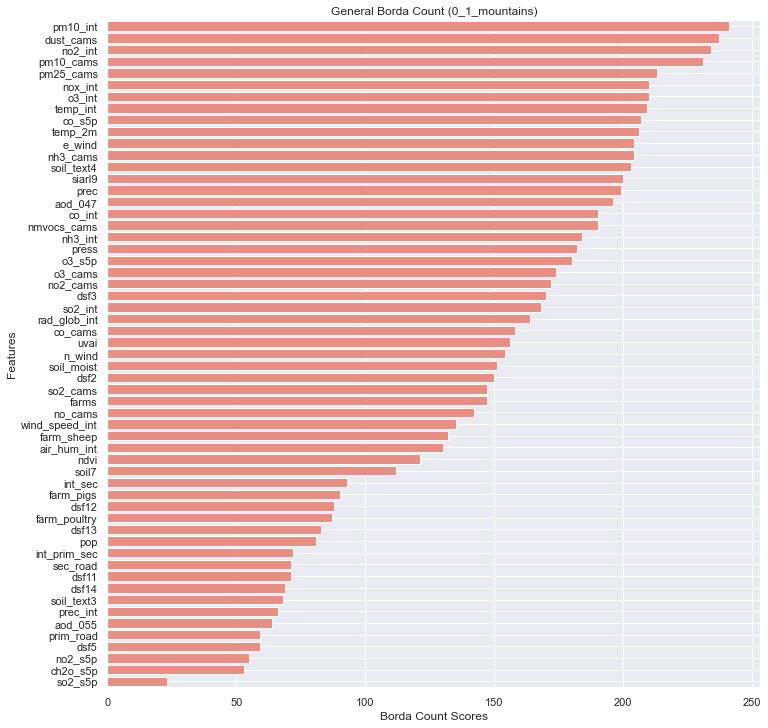
\includegraphics[scale =0.40]{images/tests/0_1_mountainspm25_st.png}}\\
\subfloat[10 Km resolution with mountains]{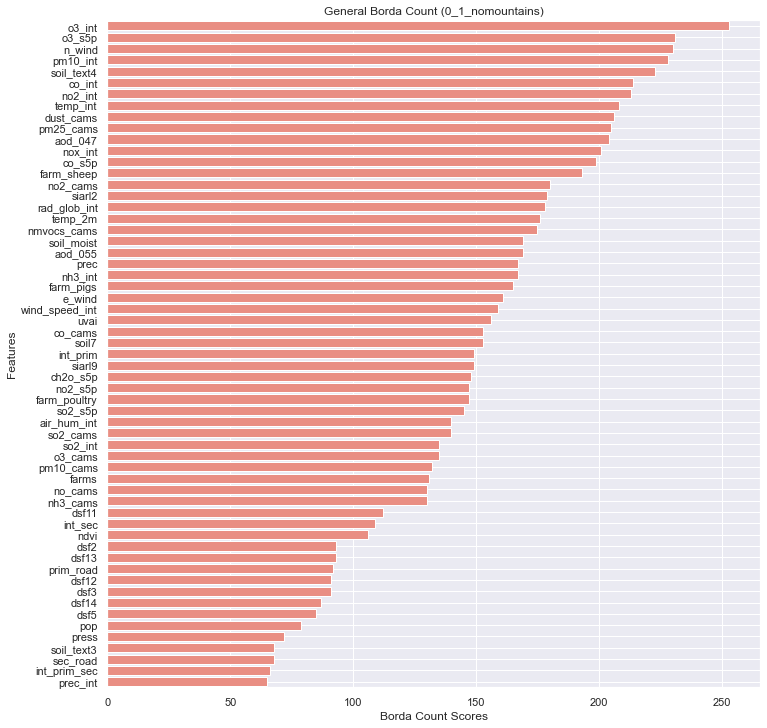
\includegraphics[scale =0.40]{images/tests/0_1_nomountainspm25_st.png}}
\caption{FS results obtained with fine particulate ('pm25\_st') as target variable and 10 km resolution. The results are averaged over the 5 periods. }
\end{figure}
\begin{figure}[H]
\centering
\subfloat[1 Km resolution with mountains]{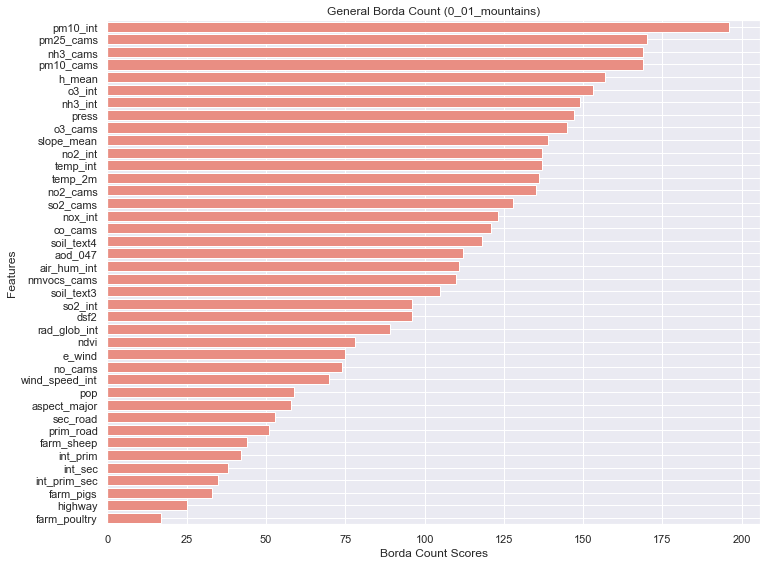
\includegraphics[scale =0.42]{images/tests/0_01_mountainspm25_st.png}}\\
\subfloat[1 Km resolution with mountains]{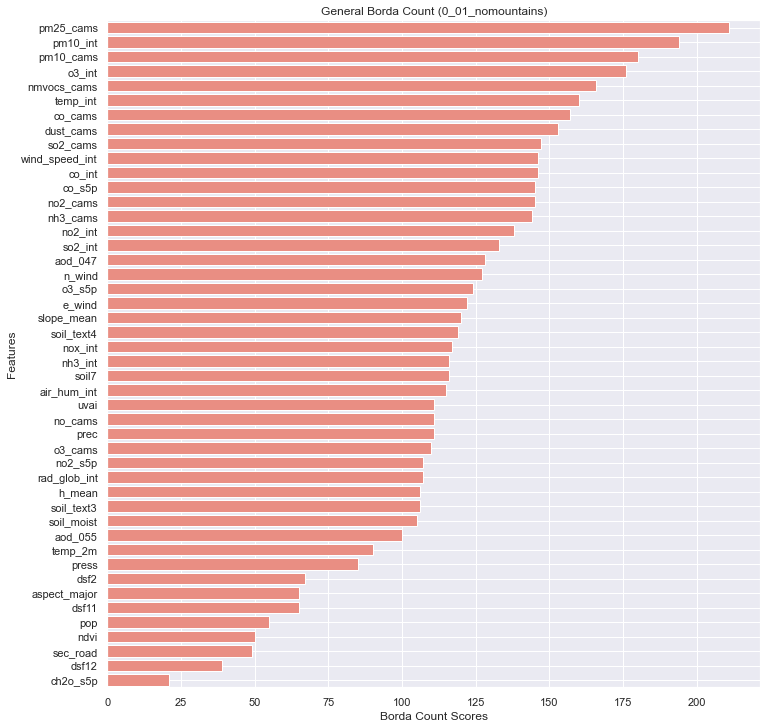
\includegraphics[scale =0.42]{images/tests/0_01_nomountainspm25_st.png}}
\caption{FS results obtained with fine particulate ('pm25\_st') as target variable and 1 km resolution. The results are averaged over the 5 periods.}
\end{figure}
\begin{figure}[H]
\centering
\subfloat[10 Km resolution with mountains]{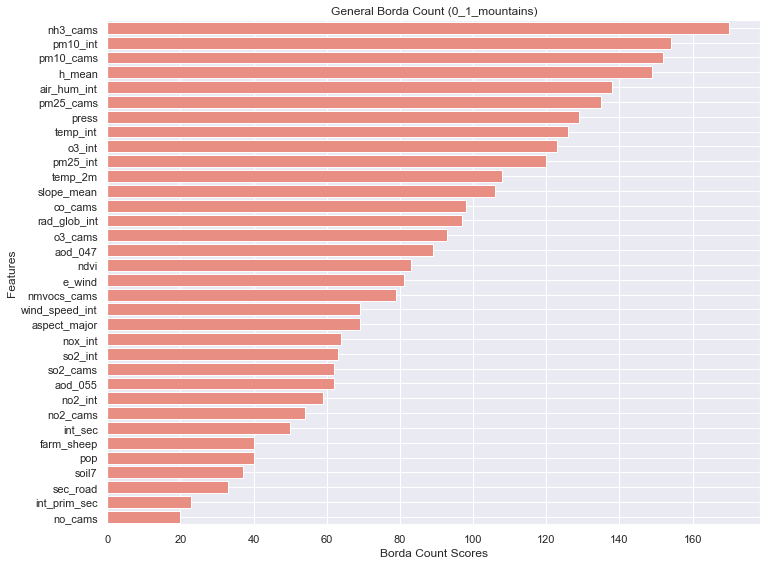
\includegraphics[scale =0.42]{images/tests/0_1_mountainsnh3_st.png}}\\
\subfloat[10 Km resolution with mountains]{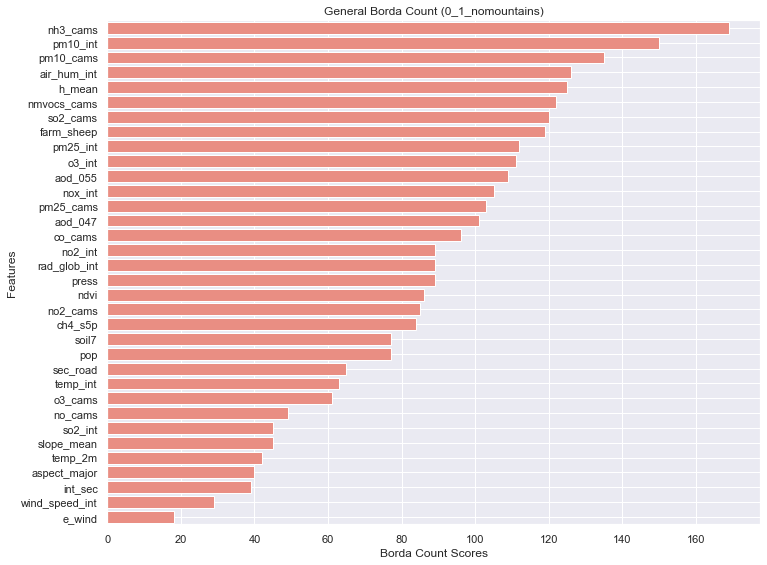
\includegraphics[scale =0.42]{images/tests/0_1_nomountainsnh3_st.png}}
\caption{FS results obtained with ammonia ('nh3\_st') as target variable and 10 km resolution. The results are averaged over the 5 periods.}
\end{figure}
\begin{figure}[H]
\centering
\subfloat[1 Km resolution with mountains]{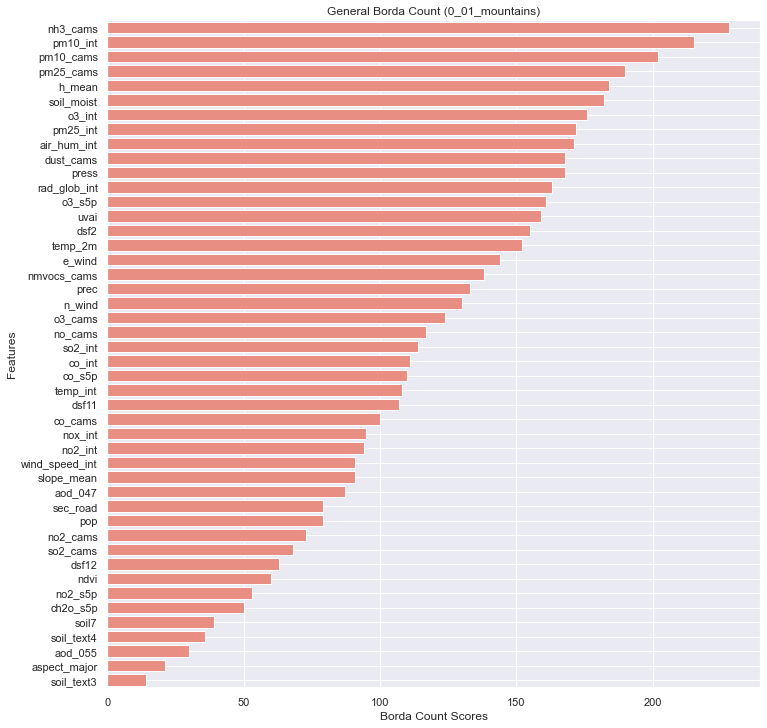
\includegraphics[scale =0.42]{images/tests/0_01_mountainsnh3_st.png}}\\
\subfloat[1 Km resolution with mountains]{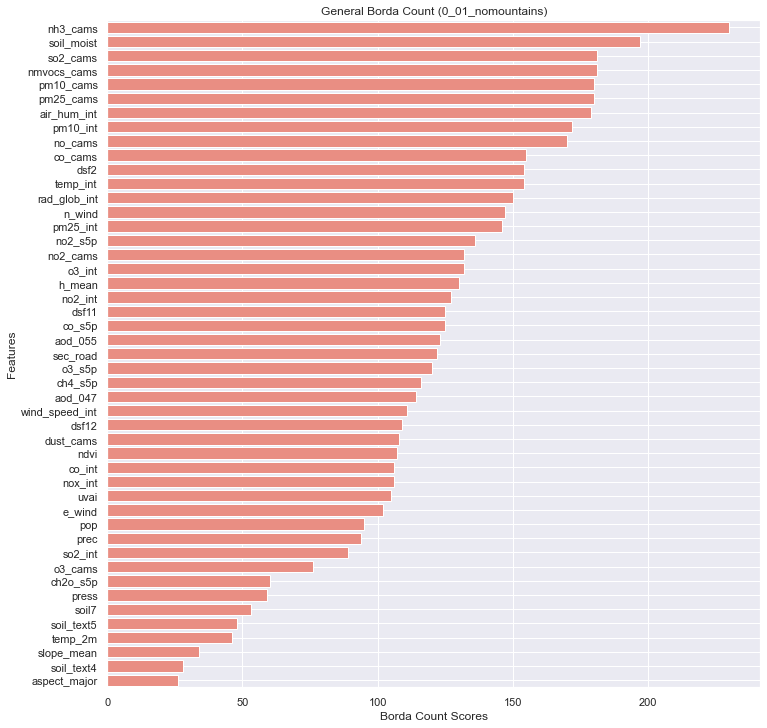
\includegraphics[scale =0.42]{images/tests/0_01_nomountainsnh3_st.png}}
\caption{FS results obtained with ammonia ('nh3\_st') as target variable and 1 km resolution. The results are averaged over the 5 periods.}
\end{figure}
\subsection{Pearson correlation index results}
\begin{figure}[H]
    \centering
    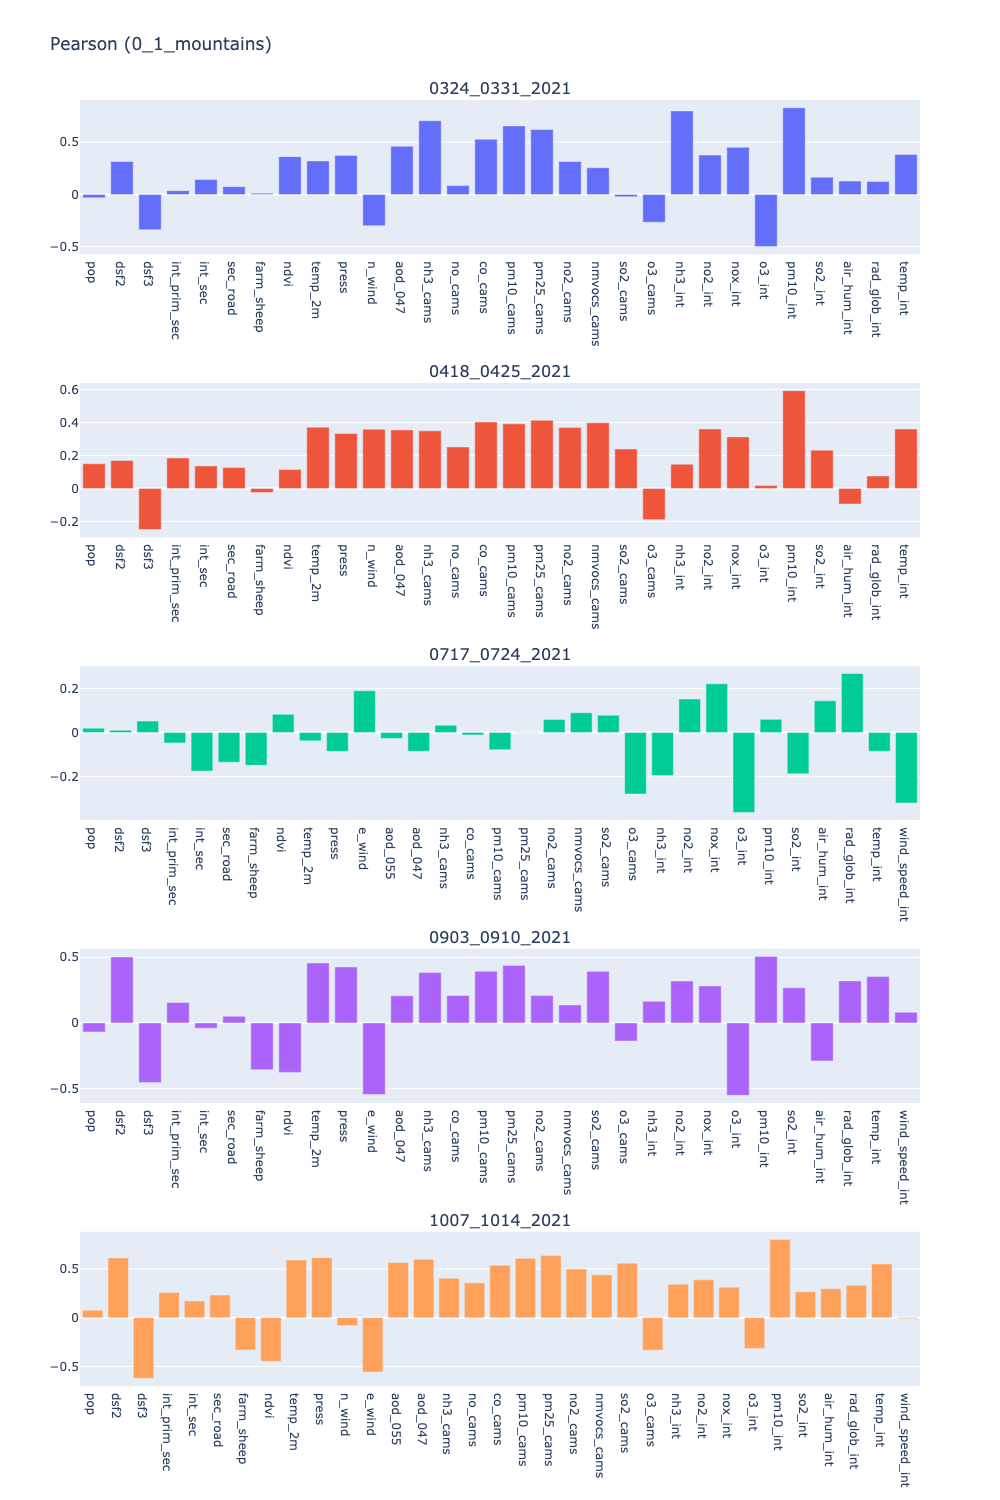
\includegraphics[scale=0.38]{images/tests/0_1_mountainspm25_st_pearson.png}
    \caption{Pearson correlation index results with respect to fine particulate ('pm25\_st') as target variable, with 10km resolution including mountains in each period. }
\end{figure}
\begin{figure}[H]
    \centering
    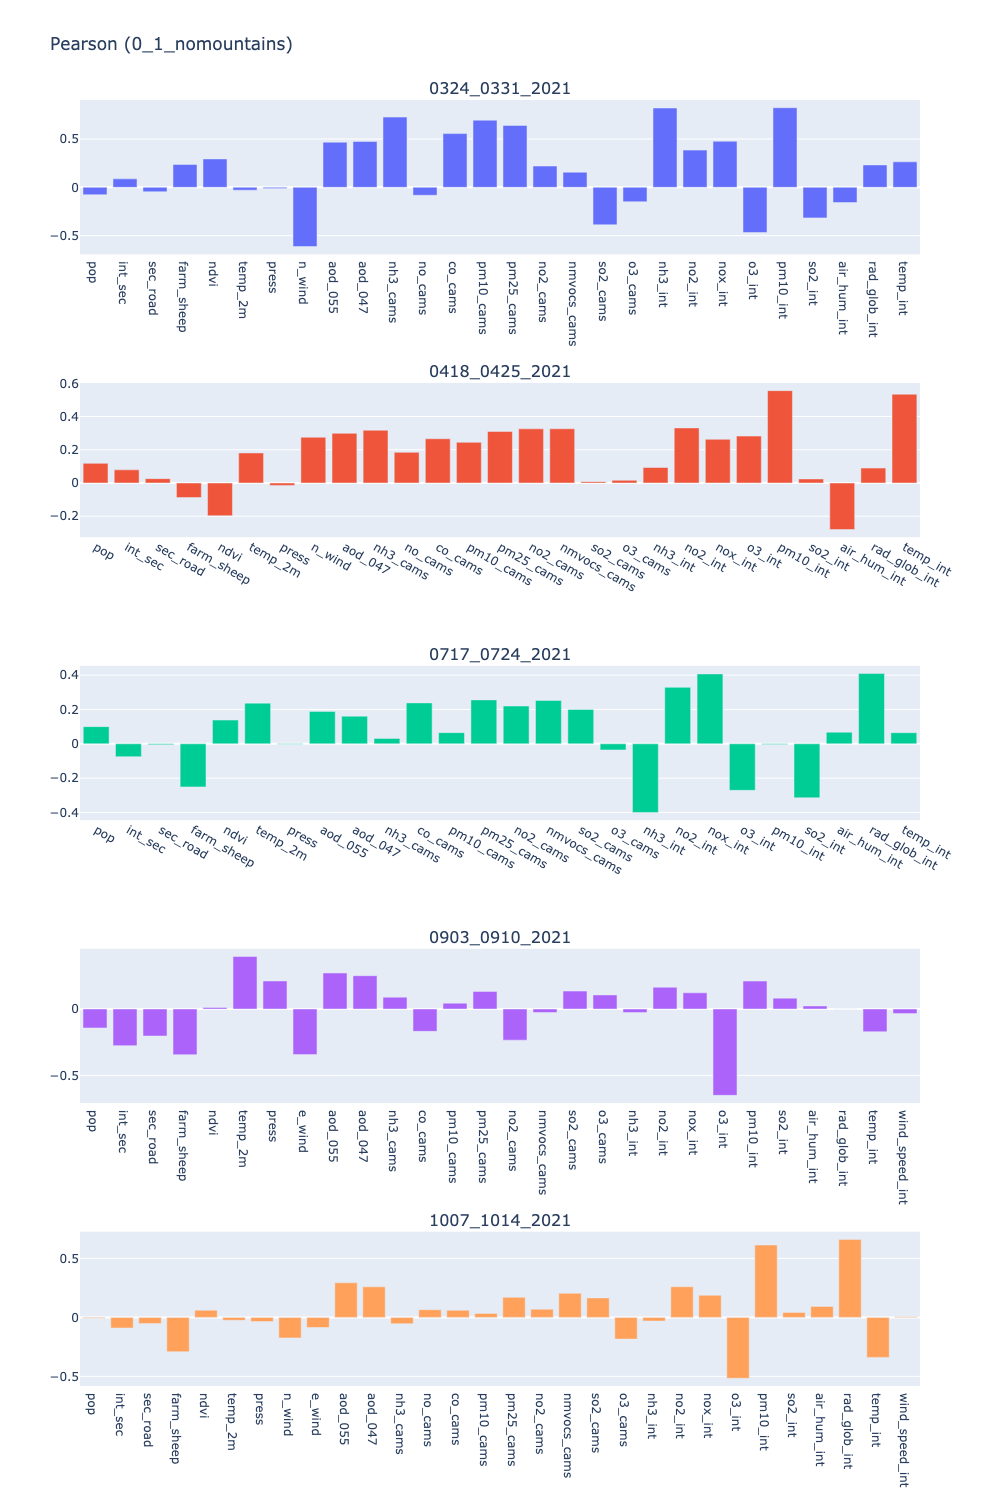
\includegraphics[scale=0.38]{images/tests/0_1_nomountainspm25_st_pearson.png}
    \caption{Pearson correlation index results with respect to fine particulate ('pm25\_st') as target variable, with 10km resolution excluding mountains in each period.}
    
\end{figure}
\begin{figure}[H]
    \centering
    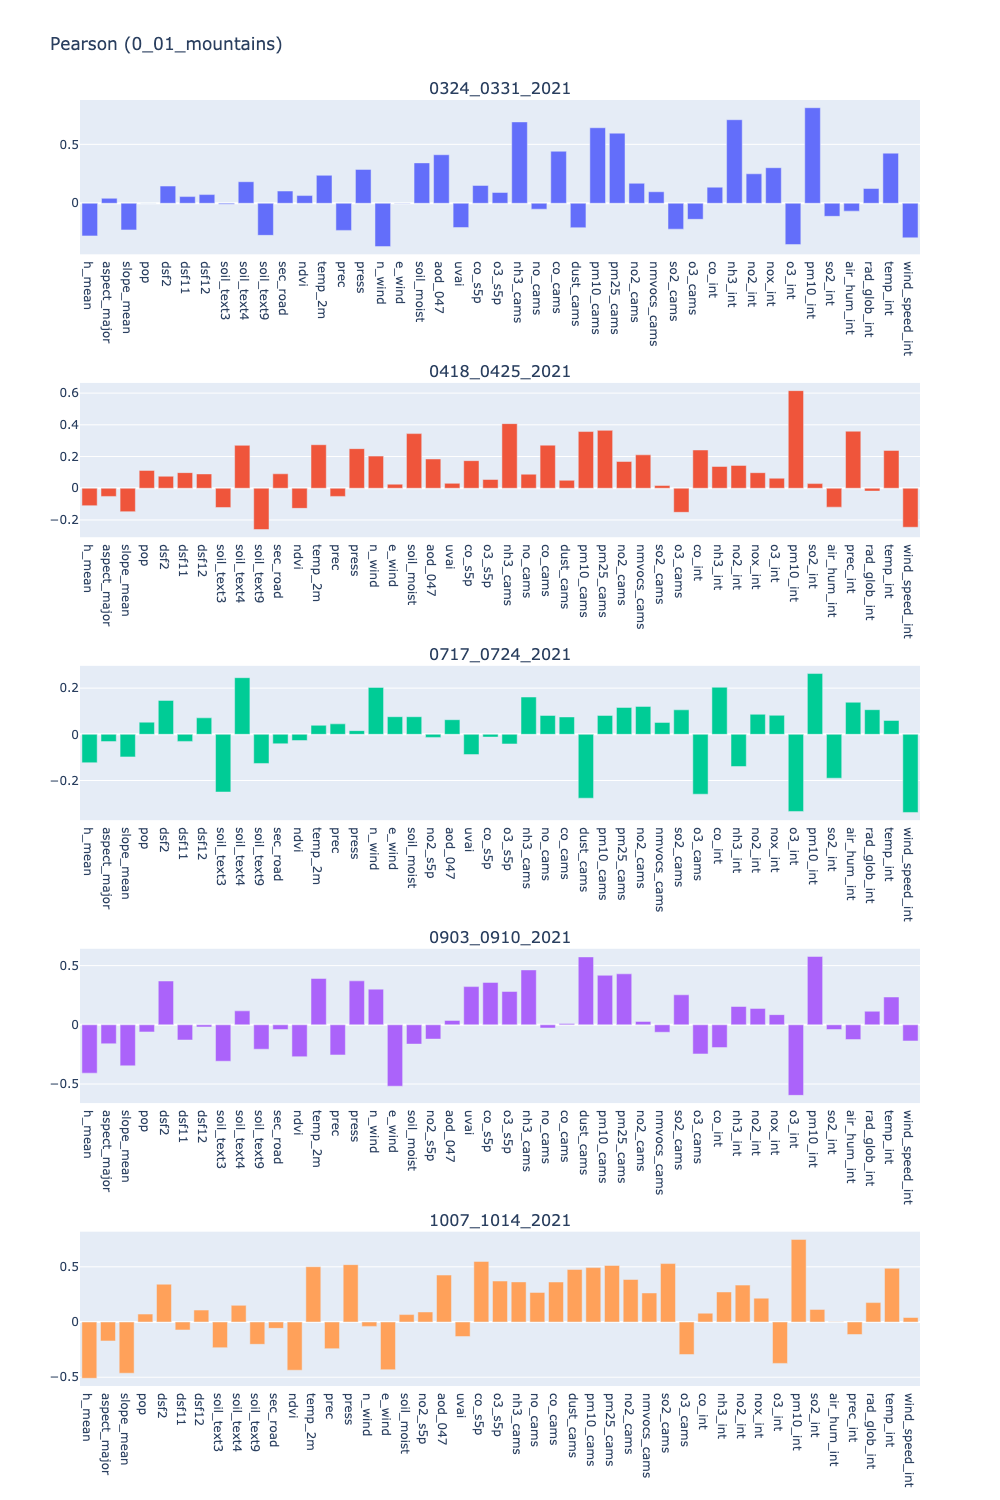
\includegraphics[scale=0.38]{images/tests/0_01_mountainspm25_st_pearson.png}
    \caption{Pearson correlation index results with respect to fine particulate ('pm25\_st') as target variable, with 1km resolution including mountains in each period.}
    
\end{figure}
\begin{figure}[H]
    \centering
    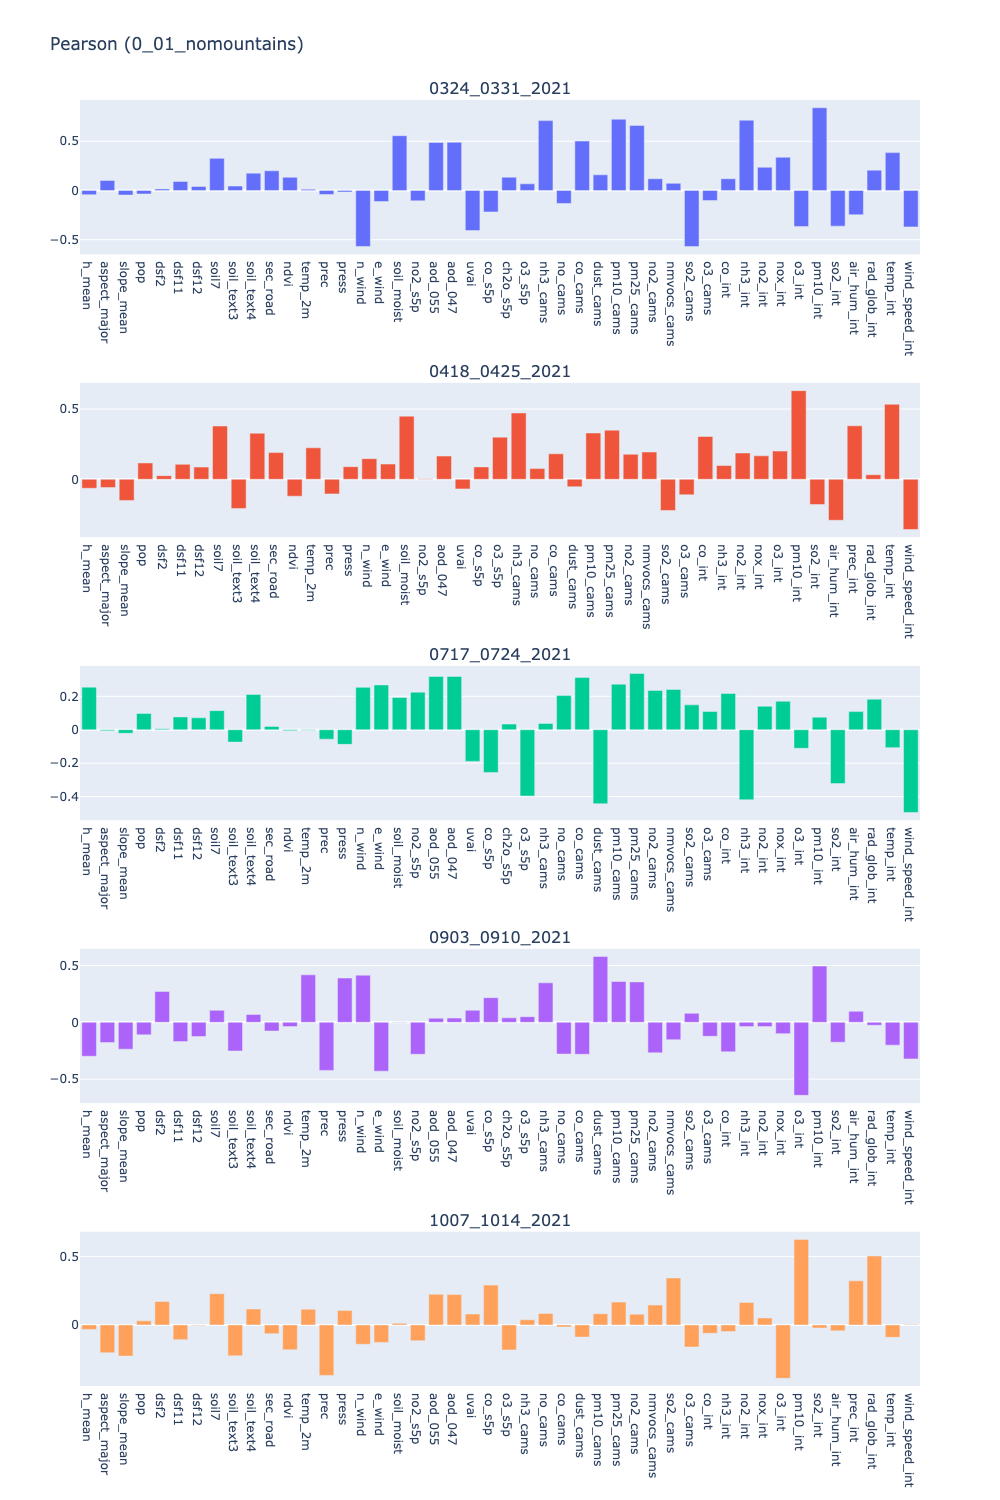
\includegraphics[scale=0.38]{images/tests/0_01_nomountainspm25_st_pearson.png}
    \caption{Pearson correlation index results with respect to fine particulate ('pm25\_st') as target variable, with 1km resolution excluding mountains in each period.}
    
\end{figure}


\begin{figure}[H]
    \centering
    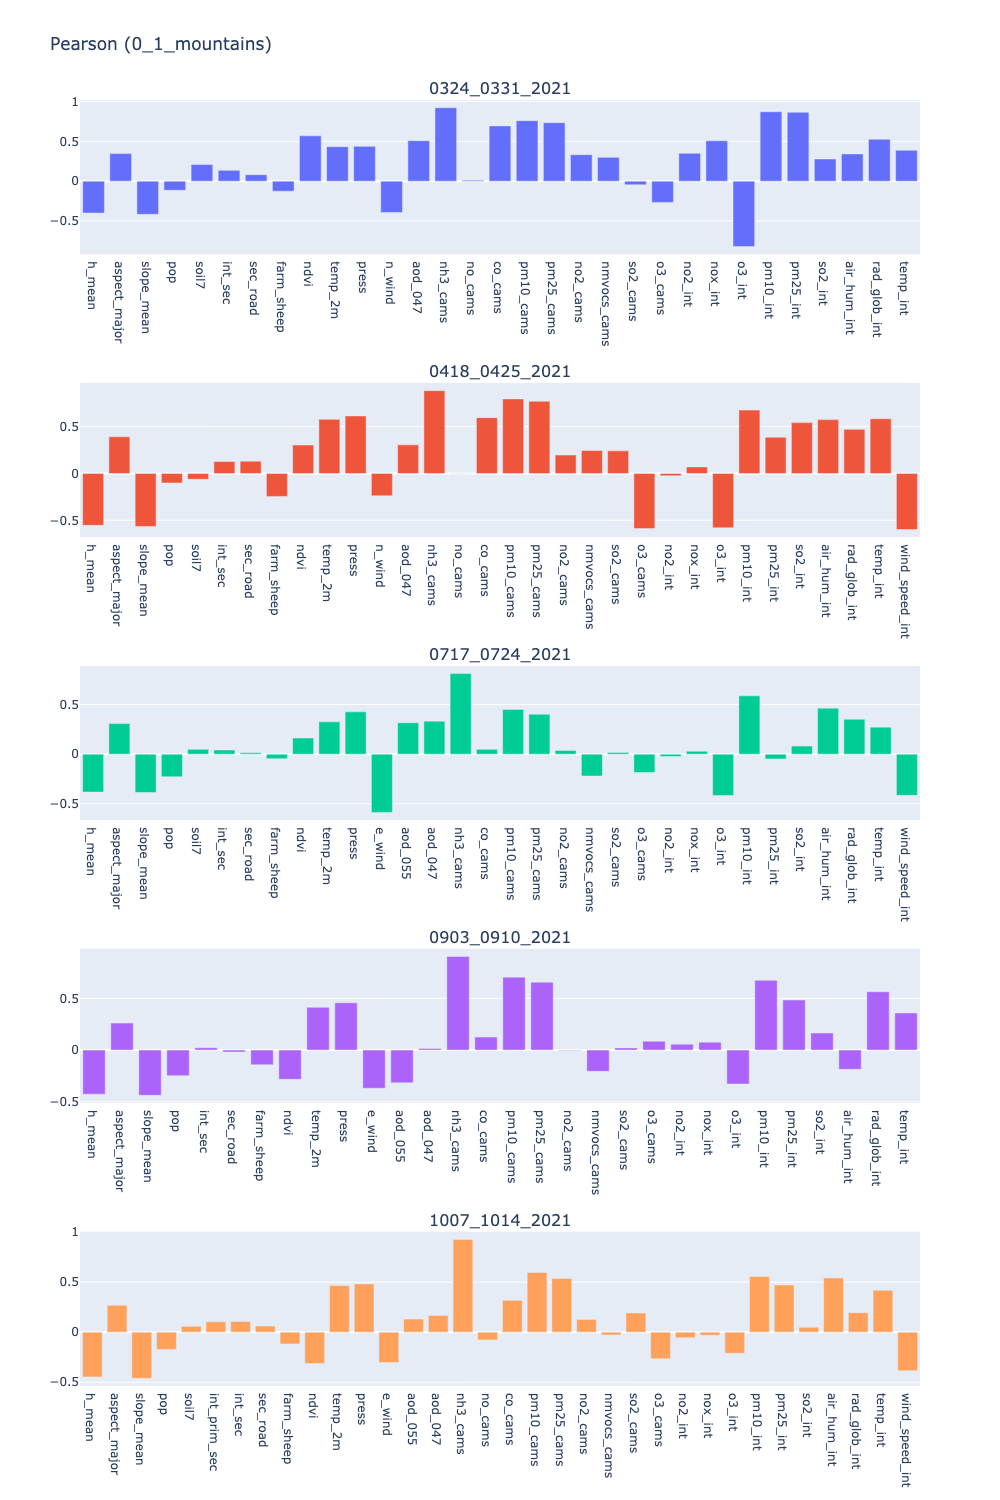
\includegraphics[scale=0.38]{images/tests/0_1_mountainsnh3_st_pearson.png}
    \caption{Pearson correlation index results with respect to ammonia ('nh3\_st') as target variable, with 10km resolution including mountains in each period.}
    
\end{figure}
\begin{figure}[H]
    \centering
    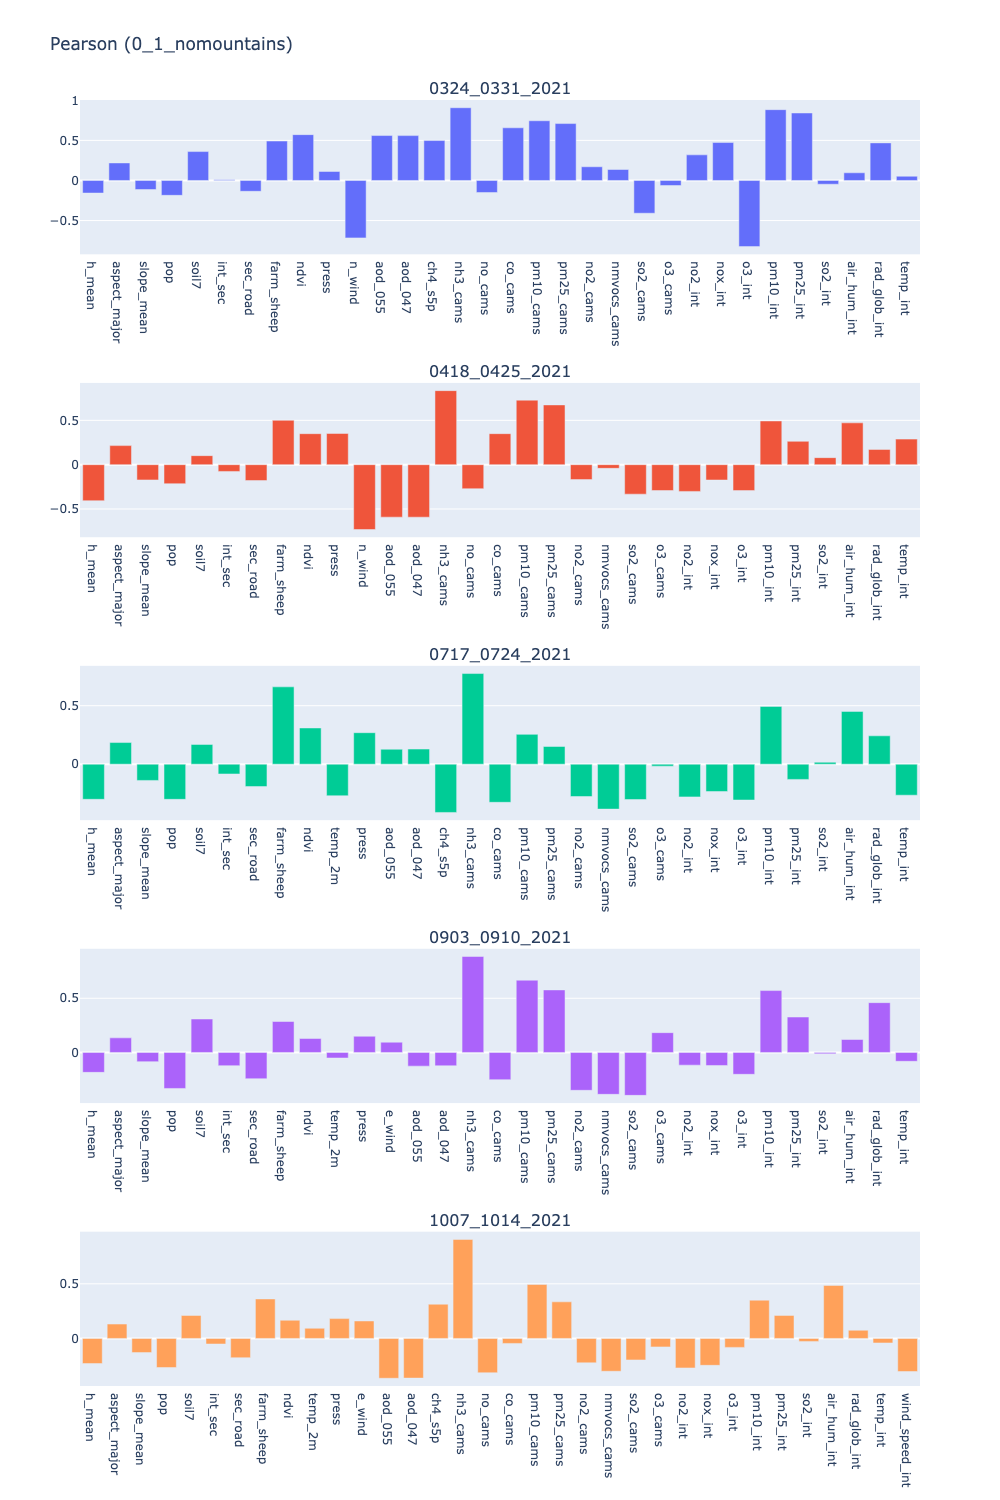
\includegraphics[scale=0.38]{images/tests/0_1_nomountainsnh3_st_pearson.png}
    \caption{Pearson correlation index results with respect to ammonia ('nh3\_st') as target variable, with 10km resolution excluding mountains in each period.}
    
\end{figure}
\begin{figure}[H]
    \centering
    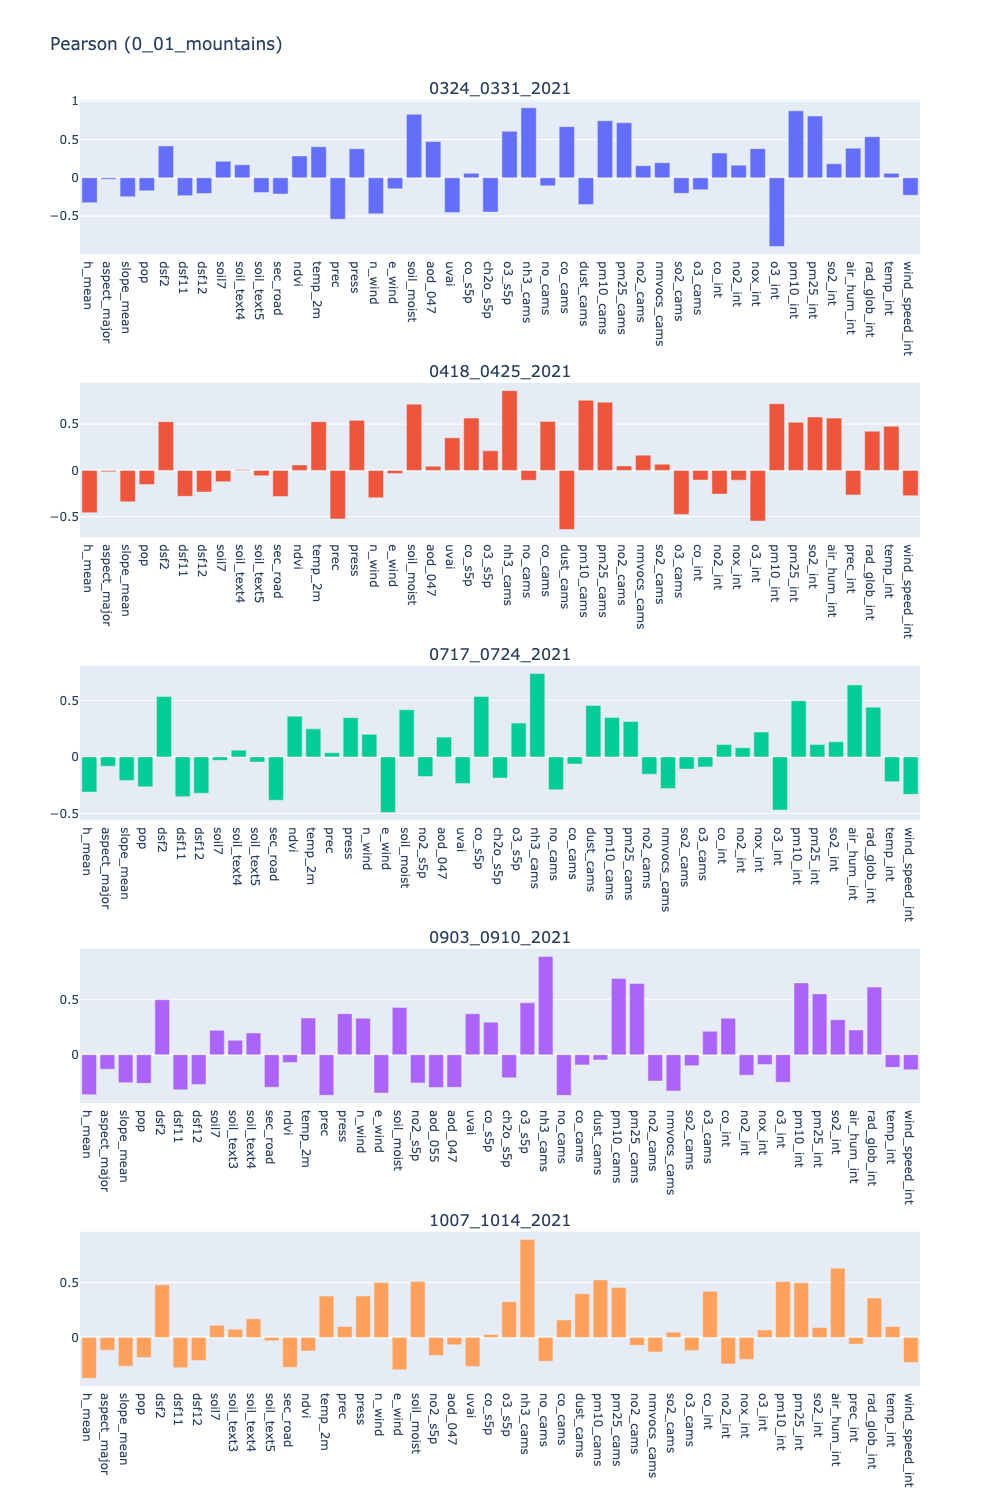
\includegraphics[scale=0.38]{images/tests/0_01_mountainsnh3_st_pearson.png}
    \caption{Pearson correlation index results with respect to ammonia ('nh3\_st') as target variable, with 1km resolution including mountains in each period.}
    
\end{figure}
\begin{figure}[H]
    \centering
    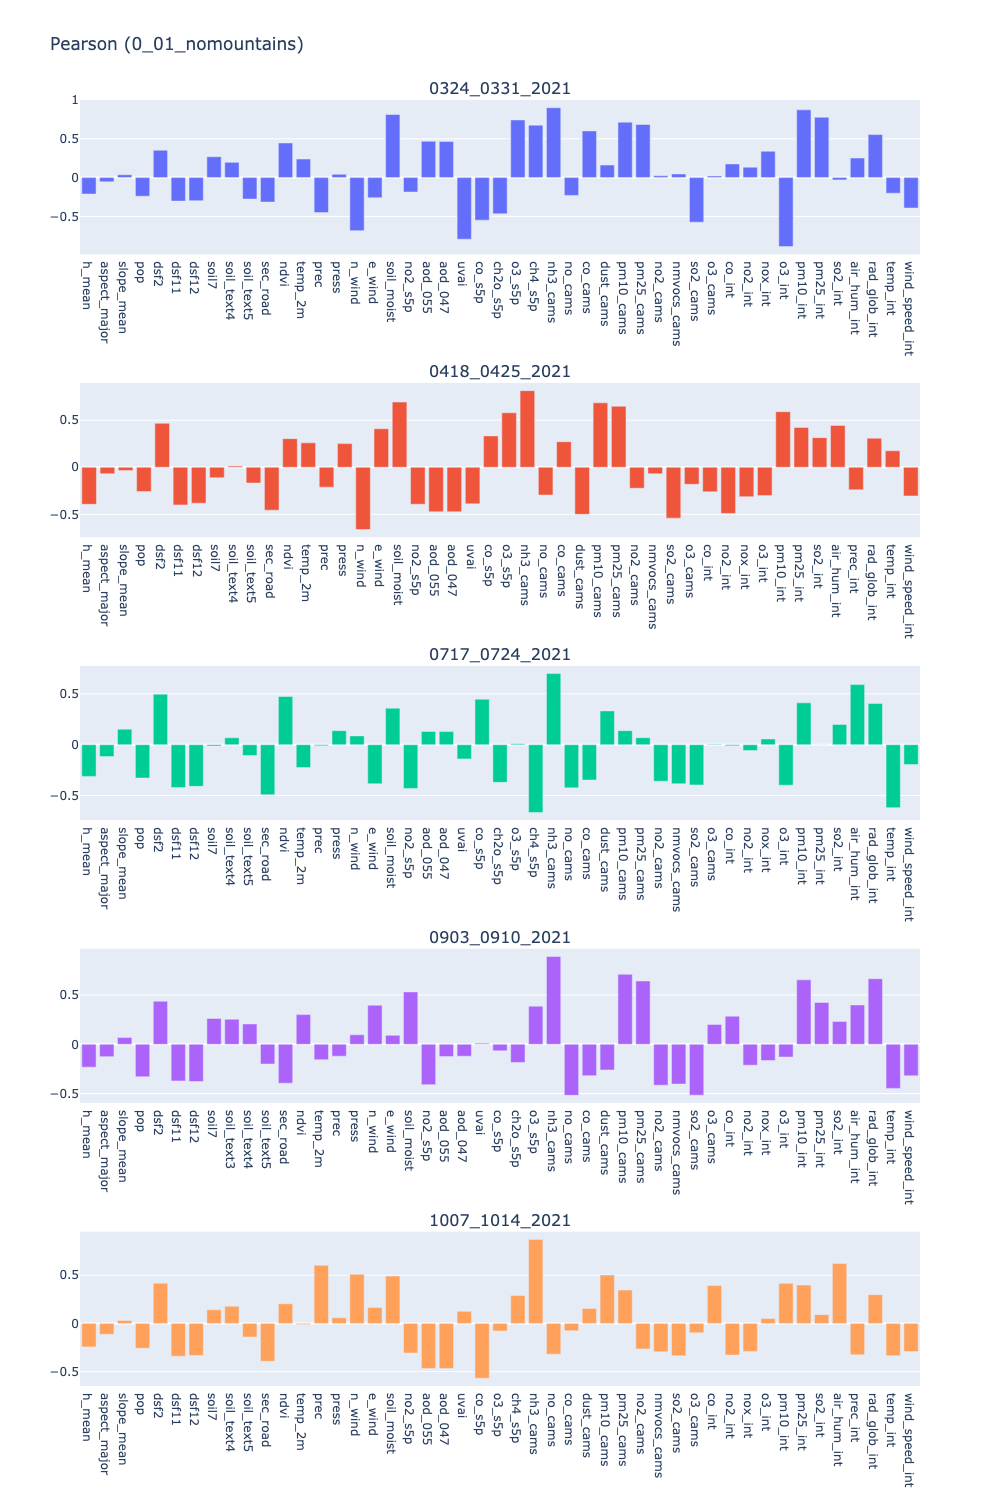
\includegraphics[scale=0.38]{images/tests/0_01_nomountainsnh3_st_pearson.png}
    \caption{Pearson correlation index results with respect to ammonia ('nh3\_st') as target variable, with 1km resolution excluding mountains in each period.}
    
\end{figure}

\section{ML models results}
\subsection{Random Forest}
\begin{table}[H]
\begin{tabular}{lrrrrr}
\toprule
 &  24/03-31/03 &  18/04-25/04 &  17/07-24/07 &  3/09-10/09 &  7/10-14/10 \\
\midrule
 MAE\_sensor ($\mu$g/m\textsuperscript{3})&        1.239 &        0.900 &        0.566 &       0.987 &       0.751 \\
RMSE\_sensor ($\mu$g/m\textsuperscript{3})&        1.768 &        1.133 &        0.745 &       1.330 &       1.013 \\
 MSE\_sensor ($\mu$g\textsuperscript{2}/m\textsuperscript{6})&        3.215 &        1.295 &        0.571 &       1.802 &       1.067 \\
  R2\_sensor &        0.883 &        0.812 &        0.722 &       0.834 &       0.858 \\
   MAE\_cams ($\mu$g/m\textsuperscript{3})&        7.800 &        6.556 &        2.110 &       3.060 &       3.478 \\
  RMSE\_cams ($\mu$g/m\textsuperscript{3})&        9.262 &        7.571 &        2.745 &       3.623 &       4.059 \\
   MSE\_cams ($\mu$g\textsuperscript{2}/m\textsuperscript{6})&       86.279 &       57.593 &        7.548 &      13.266 &      16.591 \\
    R2\_cams &       -2.147 &       -7.492 &       -2.846 &      -0.258 &      -1.096 \\
\bottomrule
\end{tabular}
\caption{Random Forest statistics for PM2.5 with 10 km resolution, including zones with mountains.}
\end{table}
\begin{table}[H]
\begin{tabular}{lrrrrr}
\toprule
 &  24/03-31/03 &  18/04-25/04 &  17/07-24/07 &  3/09-10/09 &  7/10-14/10 \\
\midrule
 MAE\_sensor ($\mu$g/m\textsuperscript{3})&        1.448 &        1.093 &        0.646 &       0.898 &       0.841 \\
RMSE\_sensor ($\mu$g/m\textsuperscript{3})&        1.940 &        1.362 &        0.868 &       1.165 &       1.080 \\
 MSE\_sensor ($\mu$g\textsuperscript{2}/m\textsuperscript{6})&        3.772 &        1.874 &        0.776 &       1.376 &       1.197 \\
  R2\_sensor &        0.872 &        0.766 &        0.683 &       0.870 &       0.793 \\
   MAE\_cams ($\mu$g/m\textsuperscript{3})&        8.230 &        7.914 &        1.386 &       3.581 &       3.744 \\
  RMSE\_cams ($\mu$g/m\textsuperscript{3})&        9.663 &        8.714 &        1.672 &       4.105 &       4.336 \\
   MSE\_cams ($\mu$g\textsuperscript{2}/m\textsuperscript{6})&       95.109 &       76.441 &        2.867 &      16.923 &      18.964 \\
    R2\_cams &       -2.312 &       -8.546 &       -0.185 &      -0.632 &      -2.373 \\
\bottomrule
\bottomrule
\end{tabular}
\caption{Random Forest statistics for PM2.5 with 10 km resolution, excluding zones with mountains.}
\end{table}
\begin{table}[H]
\begin{tabular}{lrrrrr}
\toprule
 &  24/03-31/03 &  18/04-25/04 &  17/07-24/07 &  3/09-10/09 &  7/10-14/10 \\
\midrule
 MAE\_sensor ($\mu$g/m\textsuperscript{3})&        0.251 &        0.186 &        0.147 &       0.172 &       0.132 \\
RMSE\_sensor ($\mu$g/m\textsuperscript{3})&        0.503 &        0.361 &        0.255 &       0.285 &       0.240 \\
 MSE\_sensor ($\mu$g\textsuperscript{2}/m\textsuperscript{6})&        0.283 &        0.138 &        0.066 &       0.084 &       0.059 \\
  R2\_sensor &        0.992 &        0.985 &        0.981 &       0.994 &       0.993 \\
   MAE\_cams ($\mu$g/m\textsuperscript{3})&        8.966 &        7.566 &        1.936 &       3.574 &       3.974 \\
  RMSE\_cams ($\mu$g/m\textsuperscript{3})&       10.310 &        8.472 &        2.487 &       4.099 &       4.580 \\
   MSE\_cams ($\mu$g\textsuperscript{2}/m\textsuperscript{6})&      106.414 &       71.818 &        6.213 &      16.810 &      20.988 \\
    R2\_cams &       -1.821 &       -7.099 &       -0.727 &      -0.180 &      -1.578 \\
\bottomrule
\end{tabular}
\caption{Random Forest statistics for PM2.5 with 1 km resolution, including zones with mountains.}
\end{table}
\begin{table}[H]
\begin{tabular}{lrrrrr}
\toprule
 &  24/03-31/03 &  18/04-25/04 &  17/07-24/07 &  3/09-10/09 &  7/10-14/10 \\
\midrule
 MAE\_sensor ($\mu$g/m\textsuperscript{3})&        0.347 &        0.234 &        0.156 &       0.199 &       0.146 \\
RMSE\_sensor ($\mu$g/m\textsuperscript{3})&        0.624 &        0.392 &        0.261 &       0.327 &       0.232 \\
 MSE\_sensor ($\mu$g\textsuperscript{2}/m\textsuperscript{6})&        0.411 &        0.158 &        0.069 &       0.113 &       0.054 \\
  R2\_sensor &        0.990 &        0.985 &        0.982 &       0.993 &       0.991 \\
   MAE\_cams ($\mu$g/m\textsuperscript{3})&        9.153 &        8.580 &        1.617 &       3.830 &       4.192 \\
  RMSE\_cams ($\mu$g/m\textsuperscript{3})&       10.564 &        9.294 &        1.940 &       4.382 &       4.760 \\
   MSE\_cams ($\mu$g\textsuperscript{2}/m\textsuperscript{6})&      111.721 &       86.530 &        3.766 &      19.284 &      22.676 \\
    R2\_cams &       -1.682 &       -7.131 &        0.004 &      -0.187 &      -2.674 \\
\bottomrule
\end{tabular}
\caption{Random Forest statistics for PM2.5 with 1 km resolution, excluding zones with mountains.}
\end{table}
\begin{table}[H]
\begin{tabular}{lrrrrr}
\toprule
  &  24/03-31/03 &  18/04-25/04 &  17/07-24/07 &  3/09-10/09 &  7/10-14/10 \\
\midrule
 MAE\_sensor ($\mu$g/m\textsuperscript{3})&        4.601 &        2.037 &        2.401 &       3.634 &       1.932 \\
RMSE\_sensor ($\mu$g/m\textsuperscript{3})&        5.827 &        2.809 &        3.325 &       5.074 &       2.883 \\
 MSE\_sensor ($\mu$g\textsuperscript{2}/m\textsuperscript{6})&       35.506 &        8.008 &       11.853 &      26.633 &       9.053 \\
  R2\_sensor &        0.853 &        0.815 &        0.922 &       0.854 &       0.801 \\
   MAE\_cams ($\mu$g/m\textsuperscript{3})&       14.956 &       10.748 &        8.166 &      10.326 &       9.163 \\
  RMSE\_cams ($\mu$g/m\textsuperscript{3})&       16.458 &       11.633 &       12.027 &      13.395 &      10.105 \\
   MSE\_cams ($\mu$g\textsuperscript{2}/m\textsuperscript{6})&      272.549 &      135.617 &      149.976 &     194.430 &     102.945 \\
    R2\_cams &       -0.462 &       -2.048 &        0.013 &       0.139 &      -1.066 \\
\bottomrule
\end{tabular}
\caption{Random Forest statistics for NH3 with 10 km resolution, including zones with mountains.}
\end{table}
\begin{table}[H]
\begin{tabular}{lrrrrr}
\toprule
 &  24/03-31/03 &  18/04-25/04 &  17/07-24/07 &  3/09-10/09 &  7/10-14/10 \\
\midrule
 MAE\_sensor ($\mu$g/m\textsuperscript{3})&        4.039 &        1.891 &        3.524 &       3.780 &       1.812 \\
RMSE\_sensor ($\mu$g/m\textsuperscript{3})&        5.365 &        2.496 &        4.398 &       5.358 &       2.601 \\
 MSE\_sensor ($\mu$g\textsuperscript{2}/m\textsuperscript{6})&       29.553 &        6.521 &       22.504 &      30.148 &       7.815 \\
  R2\_sensor &        0.895 &        0.829 &        0.814 &       0.848 &       0.911 \\
   MAE\_cams ($\mu$g/m\textsuperscript{3})&       15.383 &       10.758 &        8.942 &      10.304 &       9.497 \\
  RMSE\_cams ($\mu$g/m\textsuperscript{3})&       16.887 &       11.705 &       12.639 &      13.799 &      10.497 \\
   MSE\_cams ($\mu$g\textsuperscript{2}/m\textsuperscript{6})&      288.521 &      138.082 &      178.690 &     211.569 &     110.820 \\
    R2\_cams &       -0.022 &       -2.954 &       -0.236 &       0.062 &      -0.547 \\
\bottomrule
\end{tabular}
\caption{Random Forest statistics for NH3 with 10 km resolution, excluding zones with mountains.}
\end{table}
\begin{table}[H]
\begin{tabular}{lrrrrr}
\toprule
 &  24/03-31/03 &  18/04-25/04 &  17/07-24/07 &  3/09-10/09 &  7/10-14/10 \\
\midrule
 MAE\_sensor ($\mu$g/m\textsuperscript{3})&        0.450 &        0.180 &        0.505 &       0.669 &       0.345 \\
RMSE\_sensor ($\mu$g/m\textsuperscript{3})&        0.954 &        0.327 &        1.120 &       1.803 &       0.785 \\
 MSE\_sensor ($\mu$g\textsuperscript{2}/m\textsuperscript{6})&        1.065 &        0.147 &        1.861 &       4.244 &       0.732 \\
  R2\_sensor &        0.998 &        0.998 &        0.994 &       0.990 &       0.995 \\
   MAE\_cams ($\mu$g/m\textsuperscript{3})&       17.694 &       10.536 &       11.049 &      13.329 &      11.480 \\
  RMSE\_cams ($\mu$g/m\textsuperscript{3})&       18.513 &       12.046 &       16.887 &      19.503 &      12.945 \\
   MSE\_cams ($\mu$g\textsuperscript{2}/m\textsuperscript{6})&      343.112 &      145.433 &      287.761 &     382.879 &     169.030 \\
    R2\_cams &        0.227 &       -1.134 &       -0.044 &       0.124 &      -0.030 \\
\bottomrule
\end{tabular}
\caption{Random Forest statistics for NH3 with 1 km resolution, including zones with mountains.}
\end{table}
\begin{table}[H]
\begin{tabular}{lrrrrr}
\toprule
 &  24/03-31/03 &  18/04-25/04 &  17/07-24/07 &  3/09-10/09 &  7/10-14/10 \\
\midrule
 MAE\_sensor ($\mu$g/m\textsuperscript{3})&        0.483 &        0.280 &        0.526 &       0.939 &       0.386 \\
RMSE\_sensor ($\mu$g/m\textsuperscript{3})&        0.993 &        0.558 &        1.184 &       2.316 &       0.860 \\
 MSE\_sensor ($\mu$g\textsuperscript{2}/m\textsuperscript{6})&        1.199 &        0.430 &        1.556 &       6.147 &       1.121 \\
  R2\_sensor &        0.997 &        0.992 &        0.994 &       0.987 &       0.990 \\
   MAE\_cams ($\mu$g/m\textsuperscript{3})&       18.401 &       10.414 &       11.746 &      14.180 &      12.012 \\
  RMSE\_cams ($\mu$g/m\textsuperscript{3})&       19.196 &       12.126 &       17.744 &      21.241 &      13.697 \\
   MSE\_cams ($\mu$g\textsuperscript{2}/m\textsuperscript{6})&      368.858 &      147.652 &      323.418 &     456.145 &     188.650 \\
    R2\_cams &        0.136 &       -1.511 &       -0.158 &      -0.001 &      -0.060 \\
\bottomrule
\end{tabular}
\caption{Random Forest statistics for NH3 with 1 km resolution, excluding zones with mountains.}
\end{table}
\subsection{Neural Network by Keras}
\begin{table}[H]
\begin{tabular}{lrrrrr}
\toprule
 &  24/03-31/03 &  18/04-25/04 &  17/07-24/07 &  3/09-10/09 &  7/10-14/10 \\
\midrule
 MAE\_sensor ($\mu$g/m\textsuperscript{3})&        2.127 &        1.581 &        0.847 &       1.516 &       1.268 \\
RMSE\_sensor ($\mu$g/m\textsuperscript{3})&        2.643 &        2.008 &        1.046 &       1.912 &       1.591 \\
 MSE\_sensor ($\mu$g\textsuperscript{2}/m\textsuperscript{6})&        7.097 &        4.064 &        1.108 &       3.743 &       2.578 \\
  R2\_sensor &        0.750 &        0.358 &        0.408 &       0.649 &       0.672 \\
   MAE\_cams ($\mu$g/m\textsuperscript{3})&        7.800 &        6.554 &        2.113 &       3.060 &       3.478 \\
  RMSE\_cams ($\mu$g/m\textsuperscript{3})&        9.262 &        7.571 &        2.720 &       3.598 &       4.067 \\
   MSE\_cams ($\mu$g\textsuperscript{2}/m\textsuperscript{6})&       86.279 &       57.562 &        7.565 &      13.266 &      16.591 \\
    R2\_cams &       -2.147 &       -8.102 &       -3.386 &      -0.239 &      -1.158 \\
\bottomrule
\end{tabular}
\caption{Neural Network statistics for PM2.5 with 10 km resolution, including zones with mountains.}
\end{table}
\begin{table}[H]
\begin{tabular}{lrrrrr}
\toprule
 &  24/03-31/03 &  18/04-25/04 &  17/07-24/07 &  3/09-10/09 &  7/10-14/10 \\
\midrule
 MAE\_sensor ($\mu$g/m\textsuperscript{3})&        1.864 &        1.605 &        0.871 &       1.308 &       1.052 \\
RMSE\_sensor ($\mu$g/m\textsuperscript{3})&        2.257 &        1.955 &        1.100 &       1.612 &       1.327 \\
 MSE\_sensor ($\mu$g\textsuperscript{2}/m\textsuperscript{6})&        5.188 &        3.894 &        1.279 &       2.696 &       1.890 \\
  R2\_sensor &        0.826 &        0.538 &        0.457 &       0.731 &       0.653 \\
   MAE\_cams ($\mu$g/m\textsuperscript{3})&        8.243 &        7.907 &        1.383 &       3.581 &       3.744 \\
  RMSE\_cams ($\mu$g/m\textsuperscript{3})&        9.717 &        8.713 &        1.677 &       4.086 &       4.342 \\
   MSE\_cams ($\mu$g\textsuperscript{2}/m\textsuperscript{6})&       95.313 &       76.364 &        2.859 &      16.923 &      18.964 \\
    R2\_cams &       -2.281 &       -8.213 &       -0.193 &      -0.561 &      -2.351 \\
\bottomrule
\end{tabular}
\caption{Neural Network statistics for PM2.5 with 10 km resolution, excluding zones with mountains.}
\end{table}
\begin{table}[H]
\begin{tabular}{lrrrrr}
\toprule
 &  24/03-31/03 &  18/04-25/04 &  17/07-24/07 &  3/09-10/09 &  7/10-14/10 \\
\midrule
 MAE\_sensor ($\mu$g/m\textsuperscript{3})&        1.546 &        0.970 &        0.721 &       1.170 &       1.040 \\
RMSE\_sensor ($\mu$g/m\textsuperscript{3})&        1.997 &        1.340 &        0.988 &       1.528 &       1.325 \\
 MSE\_sensor ($\mu$g\textsuperscript{2}/m\textsuperscript{6})&        4.079 &        1.831 &        0.991 &       2.339 &       1.776 \\
  R2\_sensor &        0.891 &        0.798 &        0.727 &       0.839 &       0.779 \\
   MAE\_cams ($\mu$g/m\textsuperscript{3})&        8.966 &        7.567 &        1.936 &       3.574 &       3.974 \\
  RMSE\_cams ($\mu$g/m\textsuperscript{3})&       10.314 &        8.473 &        2.490 &       4.096 &       4.579 \\
   MSE\_cams ($\mu$g\textsuperscript{2}/m\textsuperscript{6})&      106.423 &       71.820 &        6.214 &      16.811 &      20.987 \\
    R2\_cams &       -1.840 &       -6.979 &       -0.735 &      -0.157 &      -1.585 \\
\bottomrule
\end{tabular}
\caption{Neural Network statistics for PM2.5 with 1 km resolution, including zones with mountains.}
\end{table}
\begin{table}[H]
\begin{tabular}{lrrrrr}
\toprule
 &  24/03-31/03 &  18/04-25/04 &  17/07-24/07 &  3/09-10/09 &  7/10-14/10 \\
\midrule
 MAE\_sensor ($\mu$g/m\textsuperscript{3})&        1.508 &        0.875 &        0.739 &       0.793 &       0.593 \\
RMSE\_sensor ($\mu$g/m\textsuperscript{3})&        1.995 &        1.174 &        0.972 &       1.002 &       0.836 \\
 MSE\_sensor ($\mu$g\textsuperscript{2}/m\textsuperscript{6})&        4.033 &        1.396 &        0.967 &       1.050 &       0.704 \\
  R2\_sensor &        0.904 &        0.868 &        0.737 &       0.937 &       0.888 \\
   MAE\_cams ($\mu$g/m\textsuperscript{3})&        9.153 &        8.581 &        1.617 &       3.830 &       4.192 \\
  RMSE\_cams ($\mu$g/m\textsuperscript{3})&       10.565 &        9.298 &        1.939 &       4.386 &       4.761 \\
   MSE\_cams ($\mu$g\textsuperscript{2}/m\textsuperscript{6})&      111.720 &       86.539 &        3.766 &      19.282 &      22.673 \\
    R2\_cams &       -1.627 &       -7.082 &       -0.006 &      -0.181 &      -2.616 \\
\bottomrule
\end{tabular}
\caption{Neural Network statistics for PM2.5 with 1 km resolution, excluding zones with mountains.}
\end{table}
\begin{table}[H]
\begin{tabular}{lrrrrr}
\toprule
 &  24/03-31/03 &  18/04-25/04 &  17/07-24/07 &  3/09-10/09 &  7/10-14/10 \\
\midrule
 MAE\_sensor ($\mu$g/m\textsuperscript{3})&        5.441 &        2.433 &        4.971 &       5.729 &       3.219 \\
RMSE\_sensor ($\mu$g/m\textsuperscript{3})&        6.896 &        3.283 &        7.496 &       7.618 &       4.613 \\
 MSE\_sensor ($\mu$g\textsuperscript{2}/m\textsuperscript{6})&       49.263 &       11.191 &       60.601 &      70.032 &      21.714 \\
  R2\_sensor &        0.785 &        0.722 &        0.618 &       0.726 &       0.722 \\
   MAE\_cams ($\mu$g/m\textsuperscript{3})&        6.660 &        4.050 &        7.537 &       6.583 &       2.601 \\
  RMSE\_cams ($\mu$g/m\textsuperscript{3})&        8.289 &        5.473 &       10.610 &       9.773 &       3.662 \\
   MSE\_cams ($\mu$g\textsuperscript{2}/m\textsuperscript{6})&       69.718 &       31.198 &      115.937 &     102.716 &      13.809 \\
    R2\_cams &        0.680 &        0.217 &        0.212 &       0.546 &       0.822 \\
\bottomrule
\end{tabular}
\caption{Neural Network statistics for NH3 with 10 km resolution, including zones with mountains.}
\end{table}
\begin{table}[H]
\begin{tabular}{lrrrrr}
\toprule
 &  24/03-31/03 &  18/04-25/04 &  17/07-24/07 &  3/09-10/09 &  7/10-14/10 \\
\midrule
 MAE\_sensor ($\mu$g/m\textsuperscript{3})&        4.625 &        2.297 &        4.749 &       5.573 &       3.139 \\
RMSE\_sensor ($\mu$g/m\textsuperscript{3})&        5.405 &        2.988 &        5.801 &       7.571 &       4.557 \\
 MSE\_sensor ($\mu$g\textsuperscript{2}/m\textsuperscript{6})&       33.849 &        9.630 &       37.672 &      58.766 &      25.848 \\
  R2\_sensor &        0.867 &        0.710 &        0.702 &       0.704 &       0.675 \\
   MAE\_cams ($\mu$g/m\textsuperscript{3})&        7.283 &        4.559 &        8.412 &       7.581 &       3.033 \\
  RMSE\_cams ($\mu$g/m\textsuperscript{3})&        8.867 &        6.016 &       11.236 &      10.874 &       4.072 \\
   MSE\_cams ($\mu$g\textsuperscript{2}/m\textsuperscript{6})&       78.979 &       36.499 &      135.704 &     123.934 &      16.818 \\
    R2\_cams &        0.710 &       -0.106 &       -0.034 &       0.425 &       0.591 \\
\bottomrule
\end{tabular}
\caption{Neural Network statistics for NH3 with 10 km resolution, excluding zones with mountains.}
\end{table}
\begin{table}[H]
\begin{tabular}{lrrrrr}
\toprule
 &  24/03-31/03 &  18/04-25/04 &  17/07-24/07 &  3/09-10/09 &  7/10-14/10 \\
\midrule
 MAE\_sensor ($\mu$g/m\textsuperscript{3})&        3.064 &        1.920 &        4.194 &       2.612 &       2.140 \\
RMSE\_sensor ($\mu$g/m\textsuperscript{3})&        3.953 &        3.010 &        5.592 &       3.497 &       2.518 \\
 MSE\_sensor ($\mu$g\textsuperscript{2}/m\textsuperscript{6})&       17.004 &        9.733 &       31.882 &      12.736 &       8.747 \\
  R2\_sensor &        0.962 &        0.861 &        0.879 &       0.968 &       0.953 \\
   MAE\_cams ($\mu$g/m\textsuperscript{3})&        8.197 &        4.031 &       10.073 &       9.247 &       4.327 \\
  RMSE\_cams ($\mu$g/m\textsuperscript{3})&       10.860 &        6.169 &       14.998 &      15.436 &       7.145 \\
   MSE\_cams ($\mu$g\textsuperscript{2}/m\textsuperscript{6})&      118.847 &       38.357 &      225.879 &     243.268 &      51.953 \\
    R2\_cams &        0.736 &        0.456 &        0.180 &       0.445 &       0.695 \\
\bottomrule
\end{tabular}
\caption{Neural Network statistics for NH3 with 1 km resolution, including zones with mountains.}
\end{table}


\begin{table}[H]
\begin{tabular}{lrrrrr}
\toprule
 &  24/03-31/03 &  18/04-25/04 &  17/07-24/07 &  3/09-10/09 &  7/10-14/10 \\
\midrule
 MAE\_sensor ($\mu$g/m\textsuperscript{3})&        1.904 &        2.287 &        3.126 &       2.743 &       3.146 \\
RMSE\_sensor ($\mu$g/m\textsuperscript{3})&        2.570 &        3.341 &        4.205 &       3.841 &       4.465 \\
 MSE\_sensor ($\mu$g\textsuperscript{2}/m\textsuperscript{6})&        6.867 &       11.579 &       18.068 &      16.405 &      21.579 \\
  R2\_sensor &        0.984 &        0.800 &        0.927 &       0.965 &       0.852 \\
   MAE\_cams ($\mu$g/m\textsuperscript{3})&        9.253 &        4.560 &       11.334 &      11.259 &       5.461 \\
  RMSE\_cams ($\mu$g/m\textsuperscript{3})&       11.641 &        6.600 &       15.831 &      17.476 &       8.145 \\
   MSE\_cams ($\mu$g\textsuperscript{2}/m\textsuperscript{6})&      135.675 &       43.816 &      257.910 &     306.085 &      67.695 \\
    R2\_cams &        0.692 &        0.254 &        0.058 &       0.342 &       0.631 \\
\bottomrule
\end{tabular}
\caption{Neural Network statistics for NH3 with 1 km resolution, excluding zones with mountains.}
\end{table}

\chapter{Appendix: comparison with CAMS model  }
\label{chap:appendixCAMS}
The comparison between the models of my results and CAMS data shows how values are very far from them. MAE for PM2.5 values is around 5 while for ammonia around 10 ug/m\textsuperscript{3}. \\
Another difference between the two models is the R\textsuperscript{2} value which assumes a negative value in most cases. It proves the presence of a big difference between training and test values. 
\begin{table}[H]
\begin{tabular}{lrrrrr}
\toprule
  &  24/03-31/03 &  18/04-25/04 &  17/07-24/07 &  3/09-10/09 &  7/10-14/10 \\
\midrule
  MAE\_cams ($\mu$g/m\textsuperscript{3})&        7.800 &        6.556 &        2.110 &       3.060 &       3.478 \\
  RMSE\_cams ($\mu$g/m\textsuperscript{3})&        9.262 &        7.571 &        2.745 &       3.623 &       4.059 \\
   MSE\_cams ($\mu$g\textsuperscript{2}/m\textsuperscript{6})&       86.279 &       57.593 &        7.548 &      13.266 &      16.591 \\
    R2\_cams &       -2.147 &       -7.492 &       -2.846 &      -0.258 &      -1.096 \\
\bottomrule
\end{tabular}
\caption{Random Forest statistics for PM2.5 at 1 km, including zones with mountains.}
\label{tab:cams1}
\end{table}
\begin{table}[H]
\begin{tabular}{lrrrrr}
\toprule
  &  24/03-31/03 &  18/04-25/04 &  17/07-24/07 &  3/09-10/09 &  7/10-14/10 \\
\midrule
   MAE\_cams ($\mu$g/m\textsuperscript{3})&       18.401 &       10.414 &       11.746 &      14.180 &      12.012 \\
  RMSE\_cams ($\mu$g/m\textsuperscript{3})&       19.196 &       12.126 &       17.744 &      21.241 &      13.697 \\
   MSE\_cams ($\mu$g\textsuperscript{2}/m\textsuperscript{6})&      368.858 &      147.652 &      323.418 &     456.145 &     188.650 \\
    R2\_cams &        0.136 &       -1.511 &       -0.158 &      -0.001 &      -0.060 \\
\bottomrule
\end{tabular}
\caption{Random Forest statistics for NH3 at 1 km, excluding zones with mountains.}
\label{tab:cams2}
\end{table}
These results are in contrast with the FS results, where the correlation between the ARPA values (target variable) and the CAMS models is one of the strongest.
From these results and the ones obtained by FS in the, we hypothesize that both pm25\_st / nh3\_st and pm25\_cams / nh3\_cams variables measure the same pollution phenomenon (figure \ref{fig:a}), but between them, there would be a bias in the samples obtained (tables \ref{tab:cams1} and \ref{tab:cams2}).\\
The model of Copernicus Atmosphere Monitoring Service provides different results than the one obtained by me since is built very differently. CAMS is built through an ensemble median, averaged by eleven European air quality forecasting systems. Therefore, the median model should perform better than the individual model products \cite{riccio2007seeking}.
Anyway, through information collected on the Copernicus website, only a limited number of ground observations are detected in the Italian territory. 
The map in figure \ref{fig:cams} includes a set of points layers representing the forecast performance of the station used by the ensemble median model of CAMS.
It can be seen that in Italy there are only 2 observations in Lombardy for PM2.5 detection.\\
Nothing was found for Ammonia.
\begin{figure}[H]
    \centering
    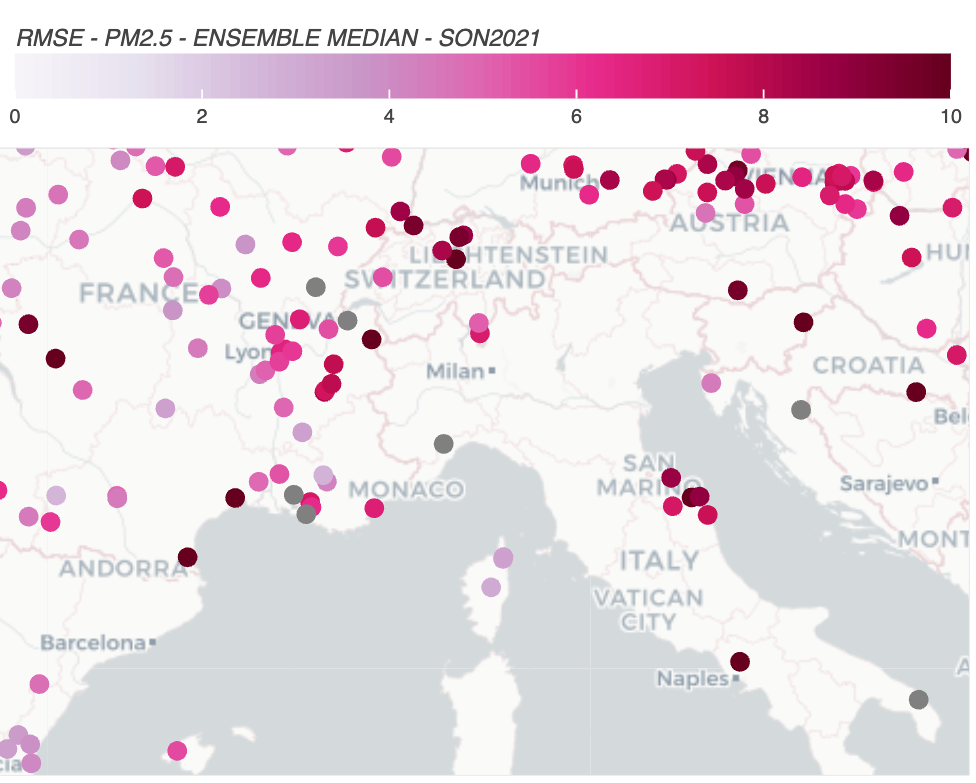
\includegraphics[scale=0.25]{images/cams_obs.png}
    \caption{Forecast performance at station and country level for the RMSE ($\mu$g/m\textsuperscript{3}) of the PM2.5 of CAMS \cite{camsobs} in 2021. 
}
    \label{fig:cams}
\end{figure}

So, by the validation results and the larger number of ground observations provided by ARPA in this data collection, we hypothesize that this model should perform better on this local scale.
\par
Based on these results, we can point out that Random Forest is more accurate than the  Neural Network model and that the performance is higher for particulate matter than ammonia estimation.\\
\begin{comment}
Random Forest indeed is one of the most preferred also in the literature statistics models for its easy configuration.
\end{comment}
